\documentclass[A_4paper,12pt]{article}
\usepackage{polski}
\usepackage{graphicx, xcolor} % Required for the inclusion of images
\usepackage{natbib} % Required to change bibliography style to APA
\usepackage{amsmath} % Required for some math elements 
\usepackage[utf8]{inputenc}
\setlength\parindent{0pt} % Removes all indentation from paragraphs
\usepackage{svg}
\usepackage{geometry}
\usepackage{afterpage}
\usepackage{caption}
\usepackage{layout}
\usepackage{tabularx}
\usepackage{wrapfig}
\usepackage{float}
\usepackage{capt-of}

\renewcommand{\labelenumi}{\alph{enumi}.} % Make numbering in the enumerate environment by 
%\usepackage{times} % Uncomment to use the Times New Roman font

\title{Laboratorium Informatyki w Medycynie \\ 3 punkt kontrolny} % Title
\author{Szymon \textsc{Gramza} 109785  \\ Przemysław \textsc{Hoffmann} 109786} % Author name

\date{23.05.2015r.} % Date for the report

\begin{document}

\maketitle % Insert the title, author and date

\begin{center}
\begin{tabular}{l r}
Prowadzący: & mgr inż. Tomasz Pawlak \\
Temat zadania: & symulator tomografu komputerowego
\end{tabular}
\end{center}

\newpage

\section{Opis problemu}
Tematem projektu zaliczeniowego jest symulator działania tomografu komputerowego.
Zgodnie z wymaganiami symulator ten powinien pozwala na:
\begin{itemize}
\item akwizycję rzutów obrazów 1D z zadanego obrazu 2D
\item prezentacje użytkownikowi tych rzutów
\item rekonstrukcję obrazów 2D z rzutów 1D przy użyciu odwrotnej transformaty Radona
\item prezentację zrekonstruowanego obrazu
\end{itemize}
Dodatkowo aplikacja pozwala w prosty sposób sterować głównymi parametrami symulatora.

\subsection{Zasada działania}
Tomografia komputerowa polega na uzyskaniu przekrojów badanego obiektu, poprzez naświetlenie obiektu wiązką promieniowania. \\
Urządzenie do tomografii komputerowej to tomograf, a uzyskany jego metodą obraz to tomogram. \\
Jako narzędzie znalazła zastosowanie w wielu dziedzinach życia, jednak najczęściej kojarzonym jest dziedzina medycyny, gdzie tomografia komputerowa służy do obrazowania ludziego ciała. Pozwala ona na wykrywanie wielu chorób już we wczesnych stadiach. \\
Do najpopularniejszych zastosowań diagnostycznych należą: diagnostyka mózgowia, udaru mózgu, badanie jamy brzusznej, miednicy, kanału kręgosłupa, oczodołów, szyi, zatok obocznychnosa, kości i stawów, klatki piersiowej i śródpiersia, a także wielu innych nie tylko standardowych, ale także bardzo specjalistycznych okolic anatomicznych.
Tomografia jest także stosowana w przemyśle do badania jakości produktów, poszukiwania wad materiałów, kontroli spoin.
\\ \\
Zasada działania tomografu komputerowego opiera się na próbie odtworzenia wewnętrznej struktury obiektu.
Dokonuje się tego poprzez wielokrotne naświetlanie, równolegle do płaszczyzny obrazowanego przekroju. \\
Informacje o tkance w trakcie badania pojedynczego przekroju uzyskujemy na podstawie pomiaru osłabienia wiązki. \\
Osłabenie promieniowania określa wzór: \\
\begin{center}
$I(S) = I(0) e^{-\int_0^S{ble}}$
\end{center}

Mała dokładność i niedoskonałość pierwszych tomografów była motywacją do kontynuowania prac nad kolejnymi wersjami.
W związku z rozwojem technologii oraz nowymi pomysłami na przestrzeni lat, tomografy sklasyfikowano na tak zwane generacje.
\subsubsection{Generacje tomografów}
Od czasów wynalezienia tomografu zmieniały się koncepcje i usprawnienia mające na celu zwiększenie ich szybkości i wydajności. \\
Poniższe zestawienie obrazuje jak zmieniało się podejście do tego zagadnienia:
\begin{itemize}
\item Generacja I - skaner składał się z pojedynczego emitera i detektora. Lampa i detektor wykonywały ruchy translacyjne i rotacyjne. \\
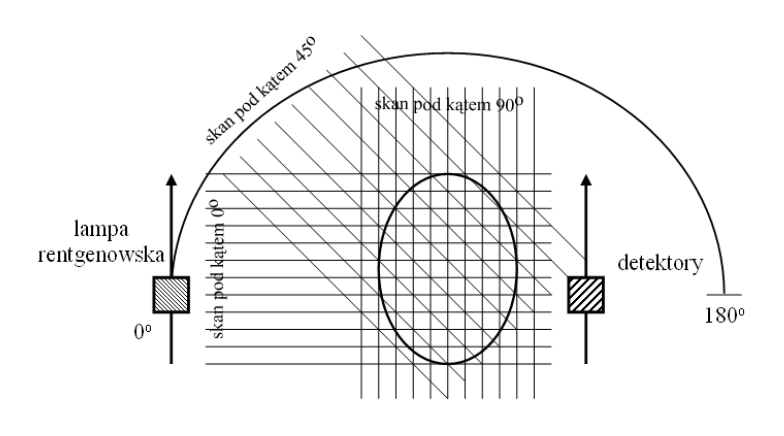
\includegraphics[scale=0.5]{1gen.png}
\item Generacja II - zwiekszono liczbę detektorów co zmniejszyło liczbę ruchów translacyjnych lampy. \\
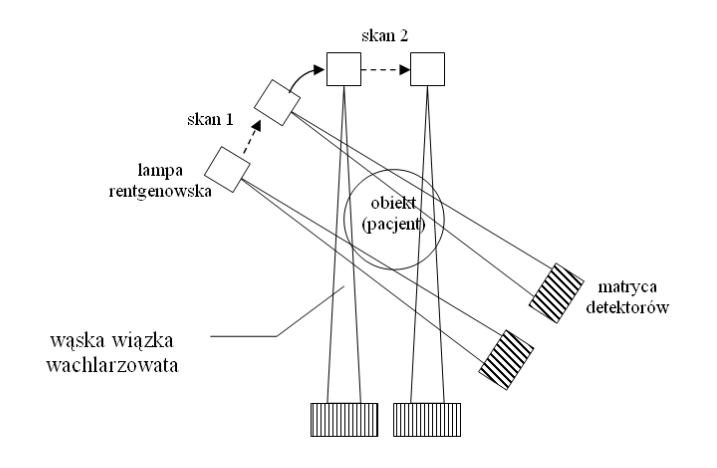
\includegraphics[scale=0.5]{2gen.png}
\item Generacja III - wyeliminowano ruch translacyjny poprzez rozmieszczenie detektorów na łuku pierścienia obracającego się razem z lampą dookoła pacjenta. \\
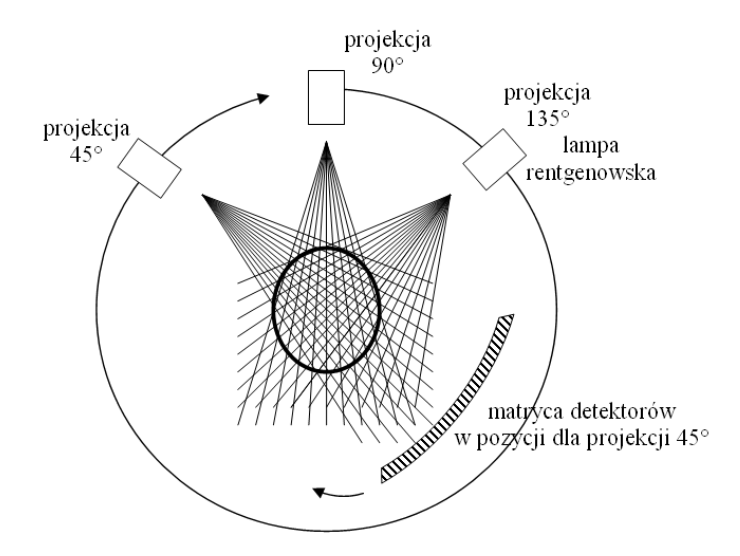
\includegraphics[scale=0.5]{3gen.png}
\item Generacja IV - detektory umieszczone zostały na stałe na pierścienu, ruch obrotowy wykonuje tylko lampa. \\
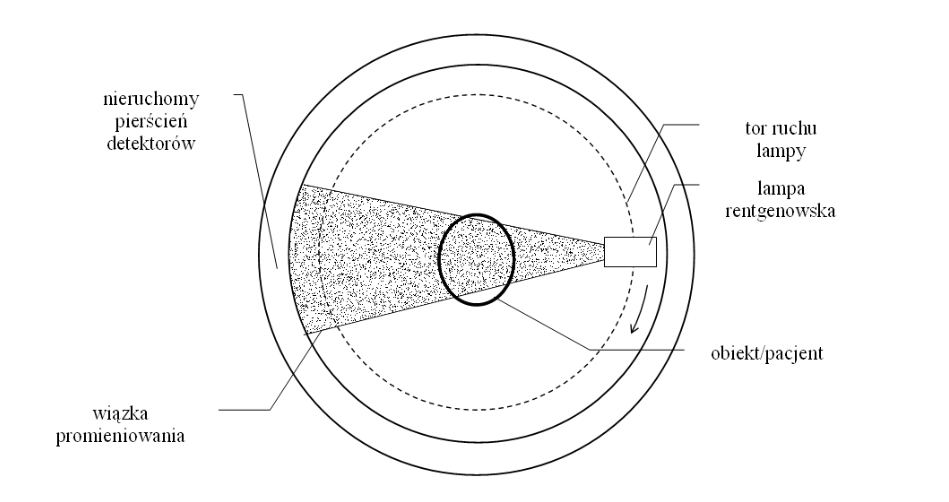
\includegraphics[scale=0.5]{4gen.png}
\end{itemize}

\section{Opis rozwiązania}
Poniżej znajduje się opis użytej technologii oraz lista zastosowanych algorytmów z wyróżnieniem na poszczególne etapy.
\subsubsection{Technologia}
Program zaimplementowany został w języku Python (wersja 2.7) z wykorzystaniem następujących bibliotek:
\begin{itemize}
\item tkinter - tworzenie, obsługa oraz zwalnianie interfejsu graficznego. 
	Pozwala na intuicyjne poruszanie się po aplikacji, wczytywanie oraz zapisywanie przetwarzanych obrazów w szczególności wczytanie obrazu do generacji sinogramu, zapis sinogramu, wczytanie sinogramu, zapis zrekonstruowanego obrazu. Dodatkowo biblioteki użyto do wygodnego sterowania najważniejszymi parametrami działania symulatora.
\item numpy - działania na macierzach, konwersje
\item math - obliczenia trygonometryczne, wartość bezwzględna
\end{itemize}


Przyjęto model tomografu o następujących parametrach:
\begin{itemize}
\item $\alpha$ - kąt o który obracany jest układ emiterów
\item $\beta$ - szerokość wiązki
\item r - odległość układu emiterów od macierzy obrazu
\item d - szerokość detektora - określa liczbę pikseli reprezentujących pojedynczy detektor
\item f - szerokość filtra
\end{itemize}

Na liczbę detektorów wpływają odległość emitera od macierzy detektorów oraz szarokość detektora.
liczba detektorów = $ \frac{2 \pi r }{d} $

Poniższy schemat obrazuje rozmieszczenie parametrów symulatora: \\
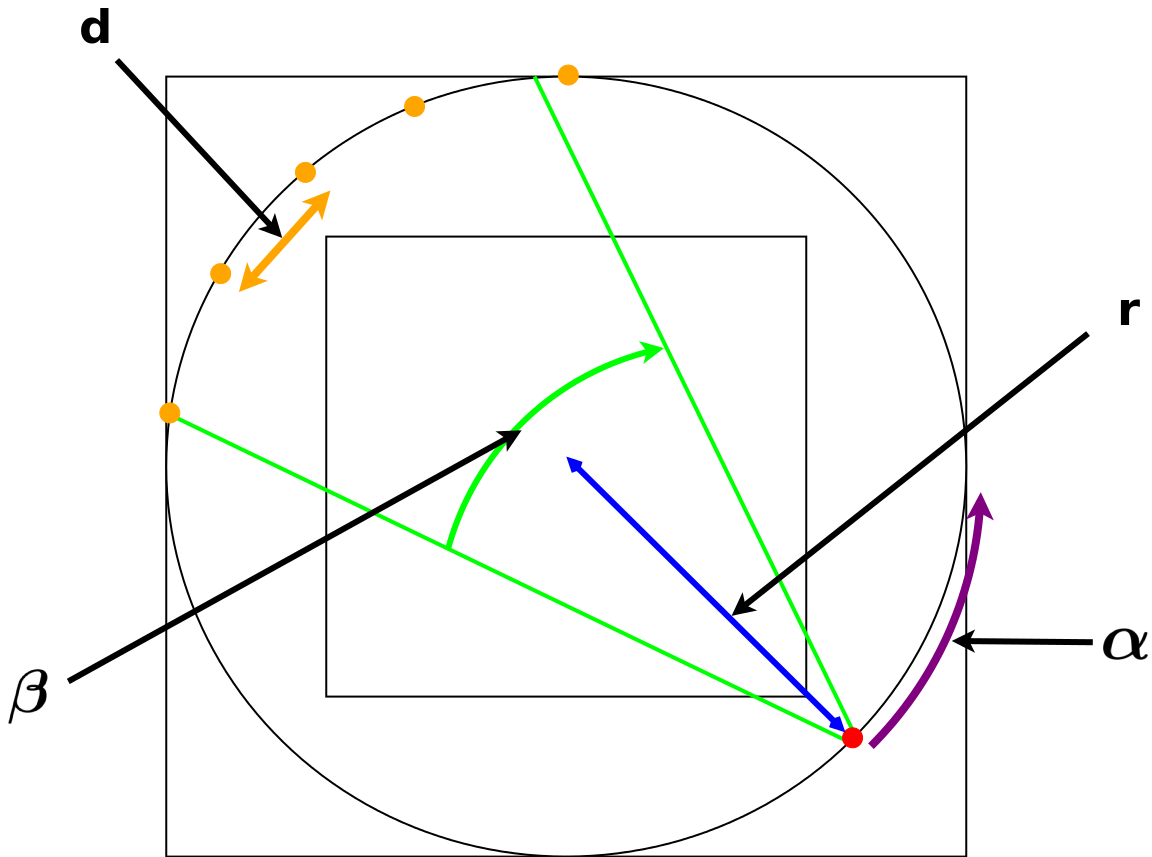
\includegraphics[scale=0.4]{schema.png}

\subsubsection{Algorytmy}
W tej sekcji znajduje się opis poszczególnych etapów przetwarzania i użytych w tym celu algorytmów.
W zakresie działania symulatora wyróżniamy głównie przetwarzanie wczytanego obrazu do postaci sinogramu, oraz rekonstrukcję otrzymanego sinogramu.
\begin{itemize}
\item W przypadku generowanie sinogramu, wykonywane są następujące kroki: \\
- oryginalny obraz zostaje wczytany w skali szarości, a następnie przechowany w pamięci w postaci lokalnej macierzy na której wykonywane są obliczenia \\
- jeśli wymiary wczytanego obrazu się różnią (tzn. szerokość $\neq$ wysokość), wówczas obraz zostaje dopełniony czarnymi pikselami na krótszym wymiarze w celu uzyskania kwadratu, otrzymujemy macierz reprezentującą w trakcie symulacji wczytany obraz (macierz A) \\
- tak otrzymana macierz kwadratowa (A) jest następnie rozszerzana do macierzy, której rozmiar zależy ściśle od parametru $r$ czyli odległości emitera od środka obrazu. \\
Jak łatwo zauważyć odległość ta nie może być mniejsza od długości przekątnej macierzy uzyskanej w pierwszym kroku. \\
W uzyskanej macierzy (B) wpisany zostaje okrąg, który odpowiada gantrze tomografu (podłużnemu tunelowi do którego wjeżdża pacjent) \\
Okrąg ten jest otrzymywany za pomocą równania parametrycznego w kartezjańskim układzie współrzędnych: \\
\[
  \begin{cases}
   x = x_0 + r \cos \alpha \\
   y = y_0 + r \sin  \alpha \\
  \end{cases}
\]
gdzie:
$r$ - odległość środka obrazu od emitera \\
$\alpha$ - kąt obrotu układu emiter - macierz detektorów \\
$x_0$ oraz $y_0$ - współrzędne środka przetwarzanego obrazu (macierz A) \\

- piksele otrzymanego okręgu są grupowane w detektory w zależności od parametru $d$ (szerokość detektorów), co zgodnie ze wzorem [numer] daje odpowiednią ilość detektorów. \\ W szczególnym przypadku ($d=1$), kazdy piksel na okręgu stanowi pojedynczy detektor. \\

- po wyznaczeniu detektorów (w przypadku gdy $d>1$ następuje wyznaczenie środka każdego z detektorów (jeden piksel) \\
- rozpoczyna się praca układu emiter-detektor, emiter startuje z pozycji 0 (obrócenie wynosi 0$^\circ$), z każdym krokiem układ obraca się o kąt $\alpha$, aż wykona pełen obrót (360$^\circ$) \\ Warto zwrócić uwagę, że wartość obrotu $\alpha$ ma bezpośredni wpływ na wysokość uzyskanego sinogramu, która wynosi $360/\alpha$ \\
- znając w każdej iteracji pozycję emitera wyznaczamy detektory na wycinku okręgu, które w danej iteracji stanowią macierz detektorów. \\
Zakres tych detektorów obrazuje przedział:
\begin{center}
$<e + 180 - (\beta/2) ; e + 180 + (\beta/2)>$
\end{center}
gdzie $e$ to aktualna pozycja emitera\\
- kolejne kroki algorytmu korzystają z algorytmu Bresenham'a. 
Służy on do rasteryzacji krzywych płaskich, czyli do jak najlepszego ich obrazowania na siatce pikseli.
W naszym zastosowaniu służy do wyznaczania pikseli obrazu, przez które przechodzi promień (pikseli leżących na odcinku od emitera do środka obrazu) oraz wyznaczenia wartości pochłoniętego promieniowania. \\
Algorytm można zastosować do rysowania odcinka, ale także okręgu czy elipsy. \\
Opis działania algorytmu: \\
- na wejściu algorytmu podajemy współrzędne punktów odcinka pomiędzy którymi mają zostać wyznaczone piksele należace do tego odcinka \\
- na podstawie różnic pomiędzy współrzędnymi na poszczególnych osiach wyznaczane są oś wiodąca oraz kierunek wyznacznia kolejnych pikseli
- oś, dla której różnica wartości współrzędnej punktu jest większa, jest osią wiodącą
- w pętli, o liczbie kroków równej różnicy współrzędnych na osi wiodącej, następuje wyznaczanie drugiej współrzędnej, natomiast krok na osi wiodącej wykonywany jest w ka żdej iteracji
- wybór wartości drugiej współrzędnej determinowany jest aktualną wartością błędu(różnicy między rzeczywistą wartością współrzędnej punktu należącego do prostej a możliwymi, całkowitymi wartościami współrzędnych pikseli), która aktualizowana jest w każdej iteracji

- do tak zaimplementowanego algorytmu Bresenham'a, w każdej iteracji (iterowanie po liście środków detektorów należących do aktualnego łuku) podawane są pozycje emitera oraz środka detektora
- dla każdej takiej pary wyznaczany jest promień (piksele należący do promienia)


TODO
- Transformata Radona
-> sumowanie wartości (posumowane/maks pikseli *255) wartość na detektorze, wartości na wszystkich środkach detektorów to jeden wiersz do sinogramu 
-> powyższe powtórzone 360/alfa razy co wpływa na rozmiar sinogramu 

\item Rekonstrukcja obrazu korzysta z wcześniejszych metod, jednak zmienia się kierunek emisji (emisja następuje od macierzy detektorów w kierunku emitera, który staje się odbiornikiem). \\
Oto lista kroków wykonywana w trakcie rekonstrukcji: \\
- W procesie rekonstrukcji bardzo ważnym elementem jest filtrowanie sinogramu, dzięki czemu obraz staje się dokładniejszy i ostrzejszy.
Filtr jest wektorem, który tworzony jest zgodnie z poniższym wzorem:
\[
 h(k) =
  \begin{cases}
   1 & \text{dla } k= 0 \\
   0 & \text{dla } k\% 2 = 0 \\
   \frac{-4/\pi^2}{k^2} & \text{dla } k\% 2 = 1 \\
  \end{cases}
\]
- tak przygotowany filtr jest stosowany na każdym wierszu sinogramu, jednak nim to nastąpi, aktualny wiersz sinogramu zostaje zmodyfikowany w taki sposób, że na krańcach wiersza zostaje doklejone lustrzane odbicie ostatnich $podłoga(n/2)$ elementów, dzięki czemu przefiltrowany wiersz sinogramu nie zmienia swojej długości \\
- samo filtrowanie polega na wyrównaniu początku filtra z początkiem filtrowanego wiersza, a następnie przemnożeniu odpowiadająych sobie pozycji i zwróceniu sumy \\
- powyższy krok jest powtarzany do (długość wiersza - długość filtra) razy \\
- przefiltrowany wiersz sinogramu w procesie rekonstrukcji wczytany zostaje na macierz detektorów \\
- następuje dodanie wartości ze środka każdego detektora do każdego piksela na drodze od środka detektora do emitera (odbywa się to opisanym wcześniej algorytmem Bresenham'a) \\
- ostatnim krokiem jest podzielenie każdej macierzy przez największą wartość w macierzy 
\end{itemize}


//może pozmieniać ale się przyda
\subsubsection{Transformata Radona}
W roku 1905 W. Radon udowodnił następujące twierdzenie: „Obraz obiektu dwuwymiarowego można zrekonstruować na podstawie nieskończonej ilości rzutów jednowymiarowych”. Rzutowanie to odpowiada wykonywaniu na obiekcie pewnej transformacji, nazywanej Transformacją Radona.
Po dokonaniu transformacji z otrzymanych wyników otrzymyje się sinogram, czyli wykres będący wizualizacją owych wyników.
Dokonanie na sinogramie Odwrotnej Transformacji Radona umożliwia zrekonstruowanie obrazu obiektu. Zrekonstruowany obraz zawierał będzie pewne zniekształcenia, lecz wraz ze wzrostem liczby projekcji powinien co raz bardziej odzwierciedlać obraz sprzed transformacji.


\section{Testy}
Przeprowadzenie testów i jakaś funkcja oceny

\section{Wnioski}
Na podstawie testów, ocena implementacji, jakie parametry optymalne w funkcji np. rozmiaru obrazu, albo ogólnie

\section{Ulepszenia}
Na podstawie wniosków co można usprawnić, co było nie tak, co może być lepsze

\section{Bibliografia}
\bibliographystyle{apalike}
\bibliography{sample}
\end{document}